\documentclass{article}

% Language setting
% Replace `english' with e.g. `spanish' to change the document language
\usepackage[UTF8]{ctex}

% Set page size and margins
% Replace `letterpaper' with `a4paper' for UK/EU standard size
\usepackage[letterpaper,top=2cm,bottom=2cm,left=3cm,right=3cm,marginparwidth=1.75cm]{geometry}

% Useful packages
\usepackage{amsmath}
\usepackage{graphicx}
\usepackage[colorlinks=true, allcolors=blue]{hyperref}

\title{MA206 Homework7}
\author{12110120 赵钊}
\date{}

\begin{document}
\maketitle


\section{第1题}
假设需要Hay、Oats、Feeding blocks、High-protein concentrate的量分别为$a$、$b$、$c$、$d$,可以根据限制条件列出限制条件方程组
\[\begin{cases}
0.5a+b+2c+6d \geq 40
\\
2a+4b+0.5c+d  \geq 20
\\
5a+2b+c+2.5d \geq 45
\\
a,b,c,d \geq 0
\end{cases} \]
求出$1.8a+3.5b+0.4c+d$的最小值即可

使用Matlab中的linprog函数求解得到,取得最小值时,$a=5$,$b=0$,$c=20$,$d=0$。因此$1.8a+3.5b+0.4c+d$的最小值为17,即达到营养条件的最小花费为17\$/week


\section{第2题}
假设4种坚果Almonds、Pecans、Cashews、Walnuts分别买$a$、$b$、$c$、$d$个单位,3种混合坚果Regular、Deluxe、Blue Ribbon分别卖掉$x$、$y$、$z$个单位,可以列出如下限制条件
\[\begin{cases}
0.25y+0.3z \leq a \leq x+y+z
\\
0 \leq b  \leq 0.25x+y+z
\\
0.3z  \leq c  \leq 0.2x+0.35y+0.5z
\\
0.4x \leq d \leq x+y+z
\\
a,b,c,d,x,y,z  \geq 0
\\
a \leq 2000
\\
b  \leq 4000
\\
c  \leq 5000
\\
d \leq 3000
\end{cases} \]
求出$0.89x+1.1y+1.8z-0.45a-0.55b-0.7c-0.5d$的最大值即可

使用Matlab中的linprog函数求解得到,取得最小值时,$a=2000$,$b=0$,$c=2000$,$d=3000$,$x=7500$,$y=0$,$z=\frac{2000}{3}$。因此$0.89x+1.1y+1.8z-0.45a-0.55b-0.7c-0.5d$的最大值为4075,即最大利润为4075


\section{第3题}
\subsection{a}
\begin{figure}[!h]
    \centering
    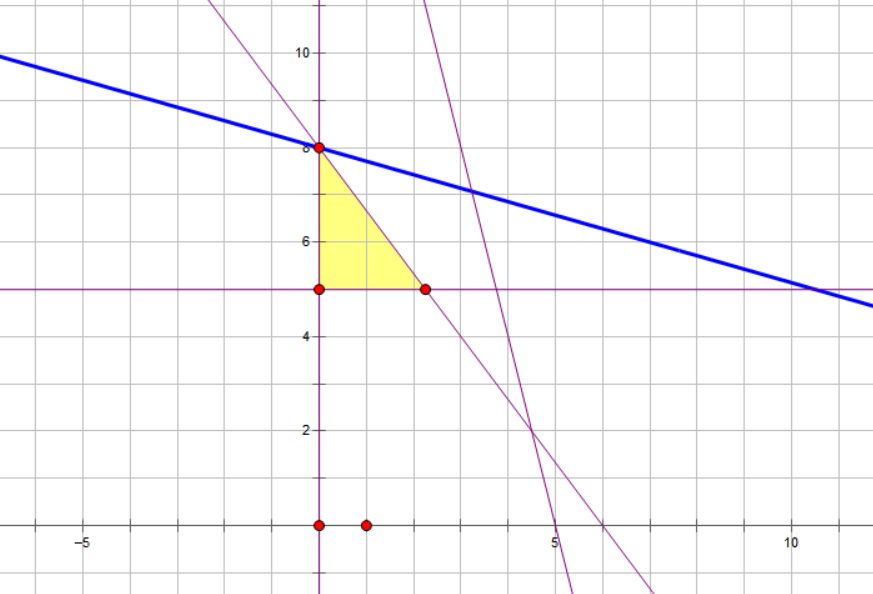
\includegraphics[width=0.75\textwidth]{pic/01.png}
    \caption{a}
\end{figure}

黄色三角形为符合限制条件的区域,假设$10x+35y=c$,则$y=-\frac{2}{7}x+\frac{c}{35}$,$c$最大时,如蓝线所示,此时$\frac{c}{35} = 8$,可得$c = 280$

\subsection{b}
\begin{figure}[!h]
    \centering
    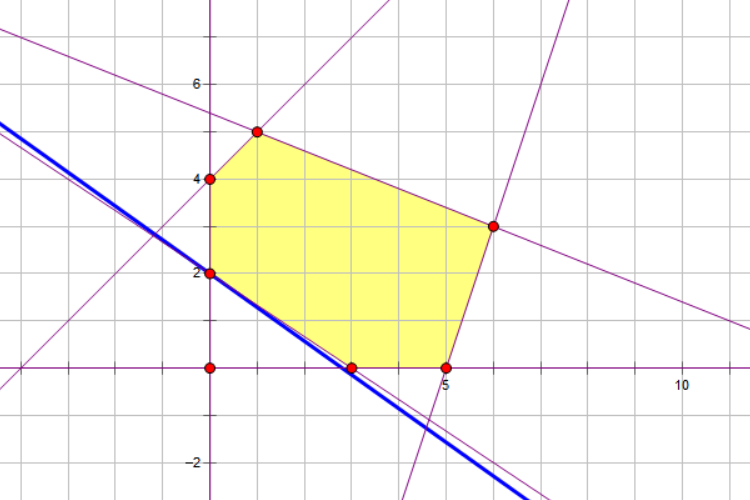
\includegraphics[width=0.65\textwidth]{pic/02.png}
    \caption{b}
\end{figure}

黄色六边形为符合限制条件的区域,假设$5x+7y=c$,则$y=-\frac{5}{7}x+\frac{c}{7}$,$c$最小时,如蓝线所示,此时$\frac{c}{7} = 2$,可得$c = 14$


\section{第4题}
\subsection{a}
使用Matlab中的linprog函数求解得到,取得最大值时,$x=0$,$y=8$因此$10x+35y$的最大值为280

\subsection{b}
使用Matlab中的linprog函数求解得到,取得最小值时,$x=0$,$y=2$因此$5x+7y$的最小值为14

\end{document}
